
\section{\unit{GridParticles}}
\label{Sec:GridParticles}

Flash-X is primarily an Eulerian code, however, there is support for
tracing the flow using Lagrangian particles. In \flashx we have
generalized the interfaces in the Lagrangian framework of the Grid
unit in such a way that it can also be used for miscellaneous 
non-Eulerian data such as tracing the path of a ray through the domain, 
or tracking the motion of solid bodies immersed in the fluid. Flash-X also
uses active particles with mass in cosmological simulations, and
charged particles in a hybrid PIC solver. Each particle has an
associated data structure, which contains fields such as its physical
position and velocity, and relevant physical attributes such as mass
or field values in active  particles. Depending upon the time advance
method, there may be other fields to store intermediate values. Also,
depending upon the requirements of the simulation, other physical variables
such as temperature \etc~ may be added to the data structure.
The \unit{GridParticles} subunit of the \unit{Grid} unit has two
sub-subunits of its own. The \unit{GridParticlesMove} sub-subunit 
moves the data structures associated with individual particles when
the particles move between blocks; the actual movement of the
particles through time advancement is the responsibility of the
\unit{Particles} unit. Particles move from one block to another
when their time advance places them outside their current
block. In AMR, the particles can also change their block through the
process of refinement and derefinement. The \unit{GridParticlesMap}
sub-subunit provides mapping between particles data and the mesh
variables. The mesh variables are either cell-centered or
face-centered, whereas a particle's position could be anywhere in the
cell. The \unit{GridParticlesMap} sub-subunit calculates the particle's
properties at its position from the corresponding mesh variable values
in the appropriate cell . When using active particles, this sub-subunit
also maps the mass of the particles onto the specified mesh variable
in appropriate cells.   The next sections describe the
algorithms for moving and mapping particles data.


\subsection{GridParticlesMove}
\label{Sec:GridParticlesMove}
\flashx has implementations of three different parallel algorithms
for moving the particles data when they are displaced from their
current block. \flashx had an additional algorithm, \code{Perfect
  Tree Level} which made use of the oct-tree structure. However,
because in all performance experiments it performed significantly
worse than the other two algorithms, it is not supported currently in
\flashx. The simplest algorithm, \code{Directional algorithm} is  
applicable only to the uniform grid when it is configured with one
block per processor. This algorithm uses directional movement of data,
and is easy because the directional neighbors are trivially known. 
The movement of particles data is much more challenging with AMR even
when the grid is not refining. Since the blocks are at various
levels of refinement at any given moment, a block may have more than one
neighbor along one or more of its faces. The distribution of blocks
based on space-filling curve is an added complication since the
neighboring blocks along a face may reside at a non-neighboring processor
The remaining two algorithmss included in \flashx implement
\code{GridParticlesMove} subunit for the adaptive mesh;  \code{Point
 to Point} and \code{Sieve}, of which only the \code{Sieve} algorithm
is able to move the data when the mesh refines. Thus even when a user
opts for the \code{PointToPoint} implementation for moving particles
with time evolution, some part of the \code{Sieve} implementation must
necessarily be included to  successfully move the data upon
refinement.   

\subsubsection{Directional Move}
\label{Sec: ug_algorithm}
The Directional Move algorithm for moving particles in a Uniform Grid 
minimizes the number of communication steps instead of minimizing
the volume of data moved. Its implementation has the following steps:
\begin{enumerate}
\item Scan particle positions.  Place all particles with their $x$
coordinate value greater than the block bounding box in the Rightmove
bin, and place those with $x$ coordinate less than block bounding box in
Leftmove bin.
\item Exchange contents of Rightbin with the right block neighbor's Leftbin
contents, and those of the Leftbin with left neightbor's Rightbin
contents.
\item Merge newly arrived particles from step 2 with those which did not move outside their original block.
\item Repeat steps 1-3 for the y direction.
\item Repeat step 1-2 for the z direaction.
\end {enumerate}

At the end of these steps, all particles will have reached their
destination blocks, including those that move to a neighbor on the
corner. \figref{Fig:ugMoveParticle} illustrates the steps in getting
a particle to its correct destination.
\begin{figure}
\begin{center}
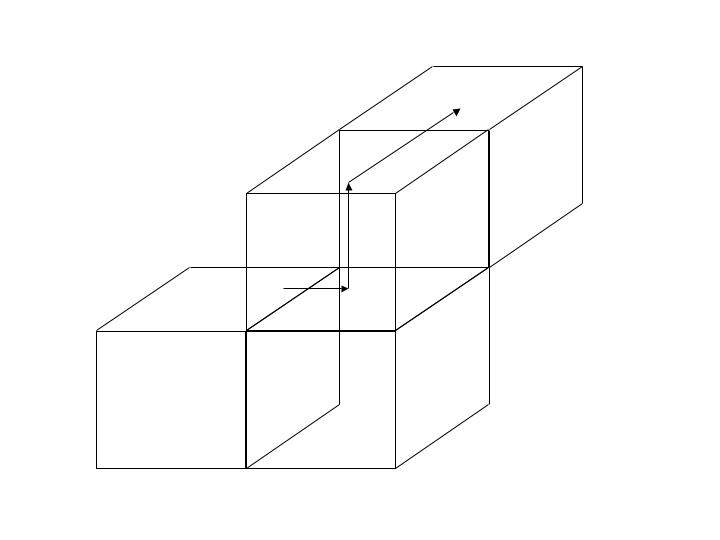
\includegraphics[width=3in]{Grid_ugMoveParticle}
\caption{\label{Fig:ugMoveParticle}
        Moving one particle to a neighbor on the corner.}
\end{center}
\end{figure}

\subsubsection {Point To Point Algorithm}
\label {Sec: ptop_algorithm}

As a part of the data cached by Paramesh, there is wealth of
information about the neighborhood of all the blocks on a
processor. This information includes the processor and block number of
all neighbors (face and corners) if they are at the same refinement
level. If those neighbors are at lower refinement level, then the
neighbor block is in reality the current block's parent's neighbor,
and the parent's neighborhood information is part of the cached
data. Similarly, if the neighbor is at a higher resolution then the
current blocks neighbor is in reality the parent of the neighbor. The
parent's metadata is also cached, from which information about all of
its children can be derived. Thus it is possible to determine the
processor and block number of the destination block for each particle.
The PointToPoint implementation finds out the destinations for every
particles that is getting displaced from its block. Particles going to
local destination blocks are moved first. The remaining particles are
sorted based on their destination processor number, followed by a
couple of global operations that allow every processor to determine
the number of particles it is expected to receive from all of the
other processors. A processor then posts asynchronous receives for
every source processor that had at least one particle to send to
it. In the next step, the processor cycles through the sorted list of
particles and sends them to the appropriate destinations using
synchronous mode of communition. 

\subsubsection{Sieve Algorithm}
\label {Sec: sieve_algorithm}
The \code{Sieve} algorithm does not concern itself with the
configuration of the underlying mesh at any time. It 
also does not distinguish between data movements due to time evolution
or regridding, and is therefore the only usable implementation when
the particles are displaced as a consequence of mesh refinement. 
The sieve implementation works with two bins, one
collects particles that have to be moved off-processor, and the other
receives particles sent to it by other processors. The following steps
broadly describe the algorithm: 
\begin{enumerate}
\item For each particle, find if its current position is on the current block
\item If not, find if its current position is on another block on the
same processor. If it is move the particle to that block, otherwise
put it in the send bin.
\item Send contents of the send bin to the designated neighbor, and
receive contents of another neighbor's send bin into my receive bin.
\item Repeat step 2 on the contents of the receive bin, and step 3
until all particles are at their destination.
\item For every instance of step 3, the designated send and receive
neighbors are different from any of the previous steps.
\end{enumerate}
In this implementation, the trick is to use an algorithm to determine
neighbors in such a way that all the particles reach their destination
in minimal number of hops. Using $MyPE+n*(-1)^{n+1}$ as the
destination processor and $MyPE+n*(-1)^{n}$ as the source processor in
modulo $numProcs$ arithmetic meets the requirements. Here $MyPE$ is
the local processor number and $numProcs$ is the number of processors.

% \subsubsection{Perfect Tree Level Algorithm}
% \label{Sec: perfectTree_algorithm}
% \code{PerfectTreeLevel} implementation exploits the oct-tree structure
% to move the data when there is no refinement. The algorithm can be
% written in four simple steps. 
% \begin {enumerate} 
% \item identify particles leaving the block
% \item move those particles up the oct-tree until they reach a level
% that is full (the level where all nodes exist)
% \item At this point the grid is reduced to Uniform Grid, apply the
% algorithm described in \secref{Sec: ug_algorithm}.
% \item move the newly arrived particles back down the tree to the
% appropriate leaves.
% \end {enumerate}
% Since each block contains complete information about its parent, and
% children it is relatively easy to navigate the
% tree. \figref{Fig:AMRParticlesNoRefine} shows the steps in the algorithm.

% \begin{figure}
% \begin{center}
% \includegraphics[width=3in]{Grid_AMRParticlesNoRefine}
% \caption{\label{Fig:AMRParticlesNoRefine}
%         Moving particles in AMR Grid when there is no refinement.}
% \end{center}
% \end{figure}


\subsection{GridParticlesMapToMesh}
\label{Sec:GridParticlesMapToMesh}
\flashx provides support for particles that can experience forces
and contribute to the problem dynamics.  These are termed
\emph{active} particles, and are described in detail in
\chpref{Chp:Particles}.  As these particles may move independently of
fluid flow, it is necessary to update the grid by mapping an attribute
of the particles to the cells of the grid.  We use these routines, for
example, during the PM method to assign the particles' mass to the
particle density solution variable \code{pden}. The hybrid PIC method 
uses its own variation for mapping appropriate physical quantities to
the mesh.

In general the mapping is performed using the grid routines in the
\code{GridParticlesMapToMesh} directory and the particle routines in
the \code{ParticlesMapping} directory.  Here, the particle subroutines
map the particles' attribute into a temporary array which is
independent of the current state of the grid, and the grid subroutines
accumulate the mapping from the array into valid cells of the
computational domain.  This means the grid subroutines accumulate the data
according to the grid block layout, the block refinement details, and
the simulation boundary conditions.  As these details are closely tied
with the underlying grid, there are separate implementations of the
grid mapping routines for UG and \Paramesh simulations.

The implementations are required to communicate information in a
relatively non-standard way.  Generally, domain decomposition parallel
programs do not write to the guard cells of a block, and only use the
guard cells to represent a sufficient section of the domain for the
current calculation.  To repeat the calculation for the next time
step, the values in the guard cells are refreshed by taking updated
values from the internal section of the relevant block.

In contrast, the guard cell values are mutable in the particle mapping
problem.  Here, it is possible that a portion of the particle's
attribute is accumulated in a guard cell which represents an internal
cell of another block.  This means the value in the updated guard cell
must be communicated to the appropriate block.  Unfortunately, the
mechanism to communicate information in this direction is not provided
by \Paramesh or UG grid.  As such, the relevant communication is
performed within the grid mapping subroutines directly.

In both \Paramesh and UG implementations, the particles' attribute is
``smeared'' across a temporary array by the generic particle mapping
subroutine.  Here, the temporary array represents a single leaf block
from the local processor.  In simulations using the \Paramesh grid,
the temporary array represents each LEAF block from the local
processor in turn.  We assign a particle's attribute to the temporary array when that
particle exists in the same space as the current leaf block.  For
details about the attribute assignment schemes available to the
particle mapping sub-unit, please refer to \secref{Sec:Particles
Mapping}.  

%Note that the particles are sorted in block
%order in the \Paramesh implementation, as this allows the particle
%mapping to be performed on a block by block basis.

After particle assignment, the \unit{Grid} sub-unit applies
simulation boundary conditions to those temporary arrays that
represent blocks next to external boundaries.  This may change the
quantity and location of particle assignment in the elements of the
temporary array.  The final step in the process involves accumulating
values from the temporary array into the correct cells of the
computational domain.  As mentioned previously, there are different
strategies for UG and \Paramesh grids, which are described in
\secref{Sec:UniformGridParticleMap} and
\secref{Sec:ParameshGridParticleMap}, respectively. 

\begin {flashtip}
The particle mapping routines can be run in a custom debug mode which
can help spot data errors (and even detect possible bugs).  In this
mode we inspect data for inconsistencies.  To use, append the
following line to the setup script:
\begin{codeseg}
-defines=DEBUG_GRIDMAPPARTICLES
\end{codeseg}
\end{flashtip}


\subsubsection{Uniform Grid}
\label{Sec:UniformGridParticleMap}

The Uniform Grid algorithm for accumulating particles' attribute on
the grid is similar to the particle redistribution algorithm described
in \secref{Sec: ug_algorithm}.  We once again apply the concept of
directional movement to minimize the number of communication steps:

\begin {enumerate}
\item Take the accumulated temporary array and iterate over all
  elements that correspond to the x-axis guard cells of the low block
  face.  If a guard cell has been updated, determine its position in
  the neighboring block of the low block face.  Copy the guard cell
  value and a value which encodes the destination cell into the send
  buffer.  %Guard cell values that have been updated must be
  %communicated to the neighboring block of the low block face.
\item Send the buffer to the low-side processor, and receive a buffer
  from the high-side processor.  For processors next to a domain
  boundary assume periodic conditions because all processors must
  participate.  If the simulation does not have periodic boundary
  conditions, there is still periodic communication at the boundaries,
  but the send buffers do not contain data.
\item Iterate over the elements in the receive buffer and accumulate
  the values into the local temporary array at the designated cells.
  It is possible to accumulate values in cells that represent internal
  cells and guard cells.  A value accumulated in a guard cell will be
  repacked into the send buffer during the next directional (y or z)
  sweep.
\item Repeat steps 1-3 for the high block face.
\item Repeat steps 1-4 for the y-axis, and then the z-axis.
\end {enumerate}

When the guard cell's value is packed into the send buffer, a single
value is also packed which is a 1-dimensional representation of the
destination cell's N-dimensional position.  The value is obtained by using an
array equation similar to that used by a compiler when mapping an
array into contiguous memory.  The receiving processor applies a
reverse array equation to translate the value into N-dimensional
space.  The use of this communication protocol is designed to minimize
the message size.

At the end of communication, each local temporary buffer contains
accumulated values from guard cells of another block.  The temporary
buffer is then copied into the solution array.



\subsubsection{Paramesh Grid}
\label{Sec:ParameshGridParticleMap}

There are two implementations of the AMR algorithms for accumulating
particles' attribute on the grid. They are inspired by a particle
redistribution algorithms \code{Sieve} and \code{Point to Point}
described  in \secref{Sec: sieve_algorithm}  and \secref{Sec:
ptop_algorithm} respectively. 

The \code{MoveSieve} implementation of the mapping algorithm uses the
same back and forth communication pattern as \code{Sieve} to minimize
the number of message exchanges.  That is, processor $MyPE$ sends to
$MyPE+n*(-1)^{n+1}$ and receives from $MyPE+n*(-1)^{n}$, where, $MyPE$
is the local processor number and $n$ is the count of the buffer
exchange round.  As such, this communication pattern involves a
processor exchanging data with its nearest neighbor processors first.
This is appropriate here because the block distribution generated by
the space filling curve should be high in data locality, \ie,
nearest neighbor blocks should be placed  on the same processor or
nearest neighbor processors.  

Similarly, the \code{Point to Point} implementation of the mapping
algorithm exploits the cached neighborhood knowledge, and uses a
judicious combination of global communications with asynchronous
receives and synchronous sends, as described in \secref{Sec:
ptop_algorithm}. Other than their communication patterns, the two
implementations are very similar as described below.

\begin {enumerate}
\item Accumulate the temporary array values into the central section
 of the corresponding leaf block.
\item Divide the leaf block guard cells into guard cell regions.
  Determine whether the neighbor(s) to a particular guard cell region
  exist on the same processor.
\item If a neighbor exists on the same processor, the temporary
  array values are accumulated into the central cells of that leaf
  block.  If the neighbor exists off processor, all temporary array
  values corresponding to a single guard cell region are copied into a
  send buffer.  Metadata is also packed into the send buffer which
  describes the destination of the updated values.
\item Repeat steps 1-3 for each leaf block.
\item Carry out data exchange with off-processor destinations as
described in the \secref{Sec: sieve_algorithm} or \secref{Sec: ptop_algorithm}
\end {enumerate}


%Step 2 and 3 are quite involved and are explained in more detail in
%the following paragraphs.

The guard cell region decomposition described in Step 2 is illustrated
in \figref{Fig:Grid_guardCell_divide}.  Here, the clear regions correspond to guard cells and
the gray region corresponds to internal cells.  Each guard cell region
contains cells which correspond to the internal cells of a single
neighboring block at the same refinement.

\begin{figure}[!ht]
\begin{center}
{\leavevmode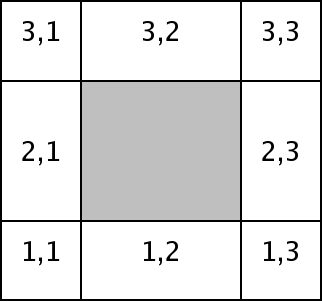
\includegraphics[width=3in]{Grid_guardCell_divide}}
\end{center}
\caption[Division of guard cells in 2-D block]{\label{Fig:Grid_guardCell_divide} A
single 2-D block showing how guard cells are divided into regions.}
\end{figure}

We use this decomposition as it makes it possible to query public
\Paramesh data structures which contain the block and process
identifier of the neighboring block at the same refinement.  However, at times
this is not enough information for finding the block neighbor(s) in a
refined grid.  We therefore categorize neighboring blocks as: Existing
on the same processor, existing on another processor and the block and
process ID are known, and existing on another processor and the block
and process ID are unknown.  If the block and process identifier are
unknown we use the \flashx corner ID.  This is a viable
alternative as the corner ID of a neighboring block can always be
determined.

The search process also identifies the refinement level of the
neighboring block(s).  This is important as the guard cell values
cannot be directly accumulated into the internal cells of another block
if the blocks are at a different refinement levels.  Instead the
values must be operated on in processes known as restriction and
prolongation (see \secref{Sec:gridinterp}).  We perform these
operations directly in the \code{GridParticlesMapToMesh} routines, and
use quadratic interpolation during prolongation.

Guard cell data is accumulated in blocks existing on the same
processor, or packed into a send buffer ready for communication.  When
packed into the send buffer, we keep values belonging to the same
guard cell region together.  This enables us to describe a whole
region of guard cell data by a small amount of metadata.  The metadata
consists of: Destination block ID, destination processor ID, block
refinement level difference, destination block corner ID (IAXIS,
JAXIS, KAXIS) and start and end coordinates of destination cells
(IAXIS, JAXIS, KAXIS).  This is a valid technique because there are no
gaps in the guard cell region, and is sufficient information for a
receiving processor to unpack the guard cell data correctly.

%The guard cell region is serialized into the send buffer in a similar
%way to \secref{Sec:UniformGridParticleMap}.  Here though, we choose to
%describe the entire guard cell region by 
%start and end coordinates for efficiency, rather than describing each
%guard cell individually.  This technique is valid as there are no gaps
%in the guard cell region.
%In order to use such an equation
%for an array, the array must be contiguous in memory.  This is not the
%case for a guard cell region, however, it can be applied because we do
%not need an actual mapping to a memory address.  All that is needed is
%a mapping to a unique 1-dimensional address, which can then be
%translated by the receiving processor into the desired N-dimensional
%cell address.  We therefore describe the entire guard cell region by 
%start and end coordinates for efficiency, rather than describing each
%guard cell individually.

We size the send / receive buffers according to the amount of data
that needs to be communicated between processors.  This is dependent
upon how the \Paramesh library distributes blocks to processors.
Therefore, in order to size the communication buffers economically, we
calculate the number of guard cells that will accumulate on blocks
belonging to another processor.  This involves iterating over every
single guard cell region, and keeping a running total of the number of
off-processor guard cells.  This total is added to the metadata total
to give the size of the send buffer required on each processor.  We use the maximum of the
send buffer size across all processors as the local size for the send
/ receive buffer.  Choosing the maximum possible size prevents
possible buffer overflow when an intermediate processor passes data
onto another processor.

After the point to point communication in step 6, the receiving
processor scans the destination processor identifier contained in each
metadata block.  If the data belongs to this processor it is unpacked
and accumulated into the central cells of the relevant leaf block.  As
mentioned earlier, it is possible that some guard cell sections do not
have the block and processor identifier.  When this happens, the
receiving processor attempts to find the same corner ID in one of its
blocks by performing a linear search over each of its leaf blocks.
Should there be a match, the guard cells are copied into the matched
block.  If there is no match, the guard cells are copied from the receive
buffer into the send buffer, along with any guard cell region
explicitly designated for another processor.  The packing and
unpacking will continue until all send buffers are empty, as indicated
by the result of the collective communication.

It may seem that the algorithm is unnecessarily complicated, however,
it is the only viable algorithm when the block and process identifiers
of the nearest block neighbors are unknown.  This is the situation in
\flashx.0, in which some data describing block and process
identifiers are yet to be extracted from \Paramesh.  
As an aside, this is different to the strategy used in Flash-X2, in
which the entire \Paramesh tree structure was copied onto each
processor.  Keeping a local copy of the entire \Paramesh tree
structure on each processor is an unscalable approach because increase
in the levels of resolution increases the meta-data memory overhead,
which restricts the size of  active particle simulations.  Therefore,
Point to Point method is a better option for
larger simulations, and significantly, simulations that run on
massively parallel processing (MPP) hardware architectures. 

In \flashx.1 we added a routine which searches non-public \Paramesh
data to obtain {\bf all} neighboring block and process identifiers.  This
discovery greatly improves the particle mapping performance because we
no longer need to perform local searches on each processor for blocks
matching a particular corner ID.

As another consequence of this discovery, we are able to experiment
with alternative mapping algorithms that require all block and process
IDs.  From \flashx.1 on we also provide a non-blocking point
to point implementation in which off-processor cells are sent directly
to the appropriate processor.  Here, processors receive messages at
incremented positions along a data buffer.  These messages can be
received in any order, and their position in the data buffer can
change from run to run.  This is very significant because the mass
accumulation on a particular cell can occur in any order, and
therefore can result in machine precision discrepancies.  Please be
aware that this can actually lead to slight variations in end-results
between two runs of the exact same simulation.  

% Finally, this
% implementation (under PttoPt subdirectory) is a proof on concept, and
% is not well tested compared to the MoveSieve implementation described
% earlier.  Also, we have no  results showing the relative performance
% of each implementation. 


%The particle positions and velocities at the next time step are calculated by
%considering both the long range and short range forces.
%The long range gravitational force between all particles is calculated 
%according to the particle-mesh (PM) technique.  In this technique, the
%gravitational acceleration on the mesh is used to update the positions and
%velocities of each particle.  
%The first stage in the technique is to 
%assign the particles' mass onto the mesh.  This gives
%a mesh-mapped particle density field in the particle density solution variable (pden).
%There are two different algorithms available for the mass assignment,
%one for UG simulations and one for \Paramesh simulations.

%This allows us to
%deduce the section in the guard cell region that needs to be copied to
%the block neighbor, and the section in the block neighbor that will
%receive the accumulated values.  


%\subsection{Example units to request}
%The stages in the PM technique and units required in 
%the Orbit simulation are as follows:
%1. Assign particles' mass to the mesh using an interpolation scheme. Different
%interpolation schemes are used depending on their accuracy and computational
%cost. The default scheme in Flash-X is Cloud-In-Cell (CIC).

%REQUESTS Particles\/ParticlesMapping\/meshWeighting\/CIC

%2. Solve Poisson's equation on the mesh in order to obtain the
%   gravitational potential.

%REQUESTS physics\/Gravity\/GravityMain\/Poisson\/Multigrid

%3. Perform a finite difference of the gravitational potential to obtain the force at each
%mesh cell.  Interpolate the forces from the cells to the particle positions
%using the same scheme as stage 1.

%REQUESTS Particles\/ParticlesMain\/active\/longRange\/gravity\/ParticleMesh

%4. Advance the particles' position and velocity.

%REQUESTS Particles\/ParticlesMain\/LeapfrogActive
